\documentclass[../thesis.tex]{subfiles}
\begin{document}
\subsection{Motivation}
\subsection{Theory}
\subsubsection{Previous Efficiency Roll-Off Models}
\subsubsection{Exciton Dynamics}
\subsubsection{Polaron Dynamics}
\subsubsection{Exciton Quenching in Photoluminescence}
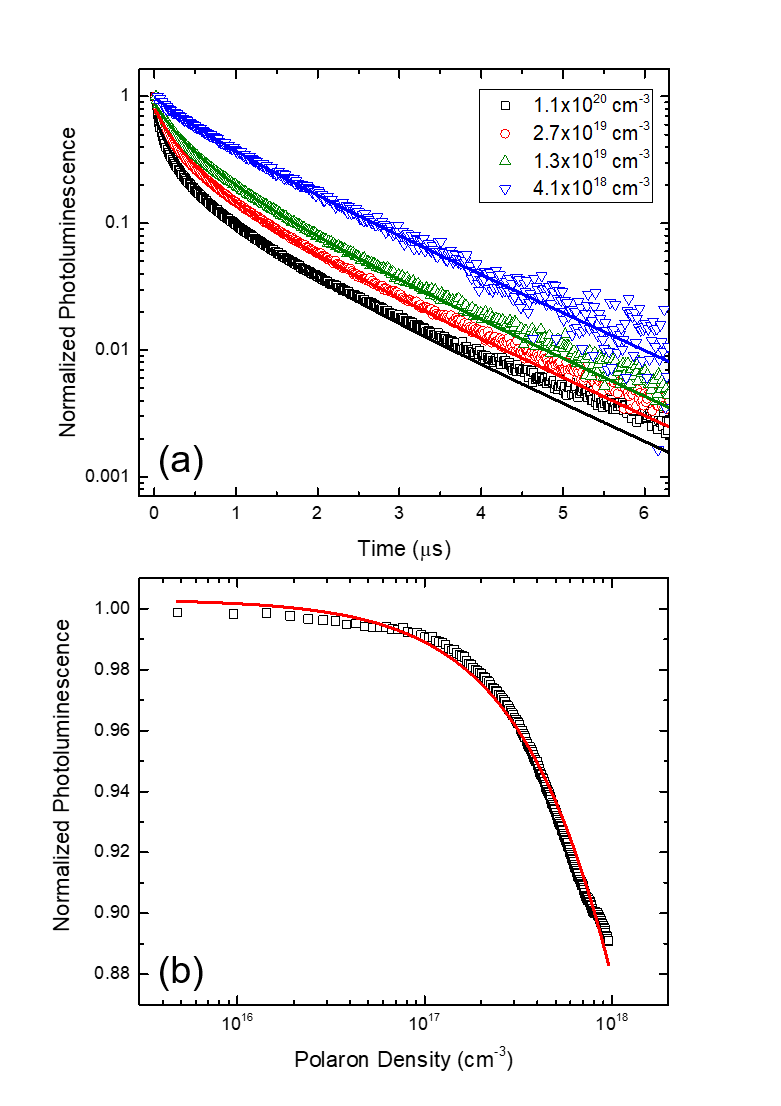
\includegraphics[scale=.25]{unified/PL_fitting}
\subsubsection{Transient Electroluminescence}
\subsubsection{Efficiency Analysis}
\subsection{Experimental Details}
\subsection{Application to Devices}
\subsubsection{Overview of Approach}
\subsubsection{Initializing Parameters with Quenching Only Steady-State Model}
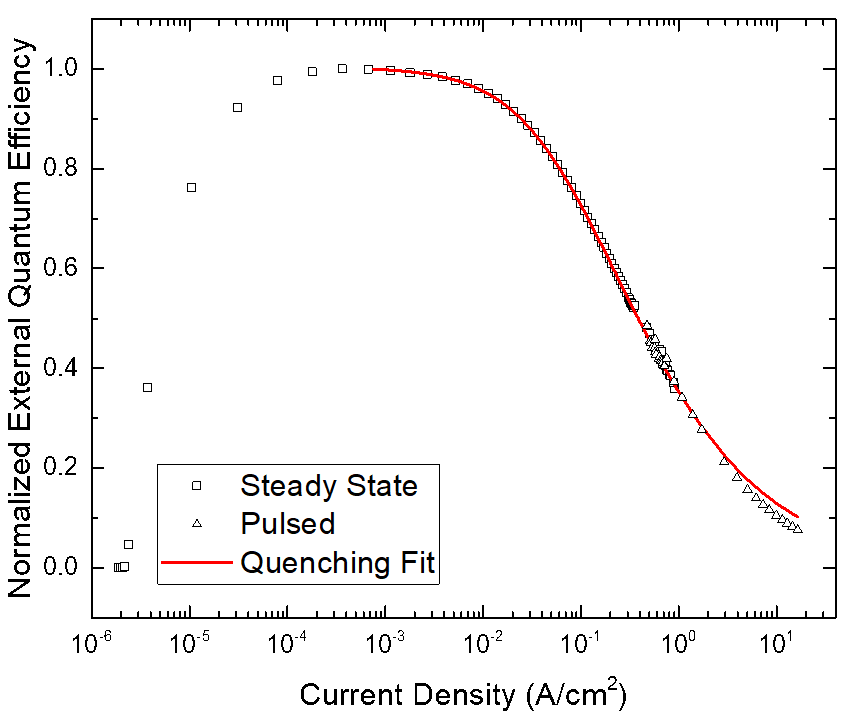
\includegraphics[scale=.25]{unified/rollOffFit}
\subsubsection{Transient Modeling}
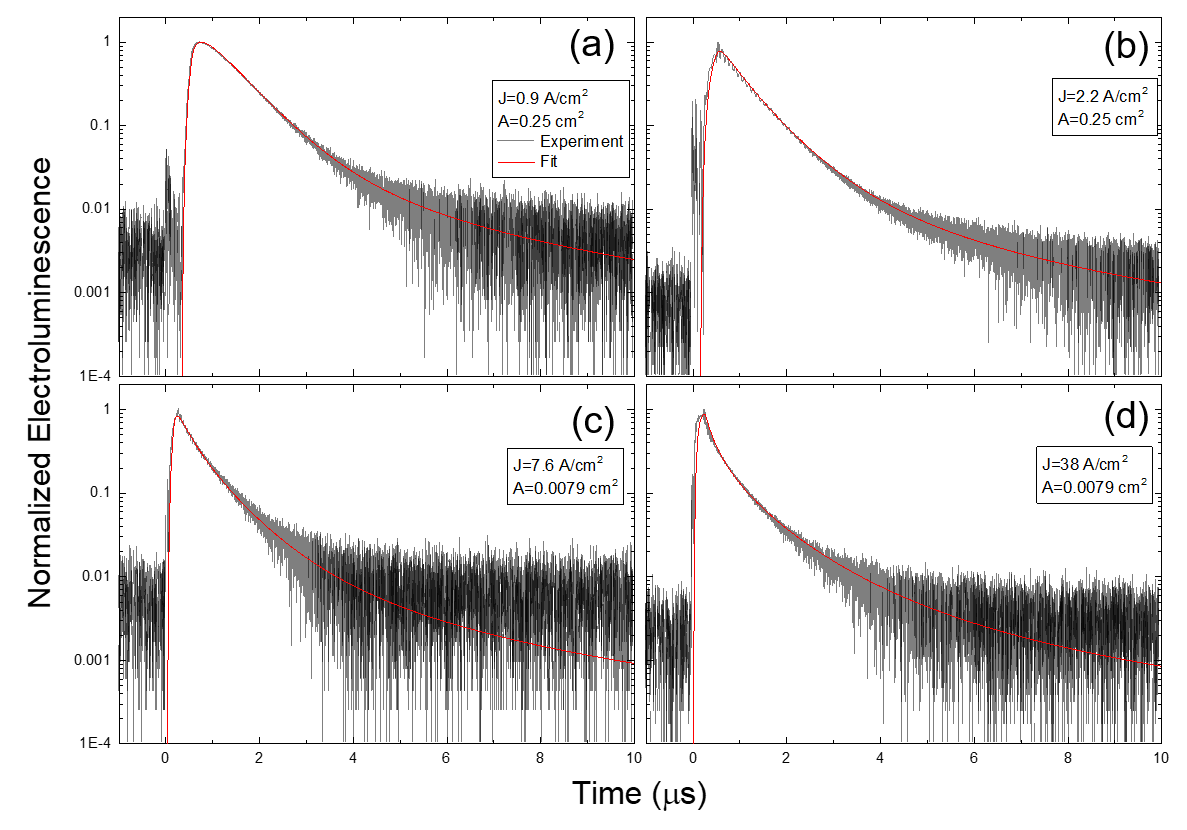
\includegraphics[scale=.25]{unified/transientFits}
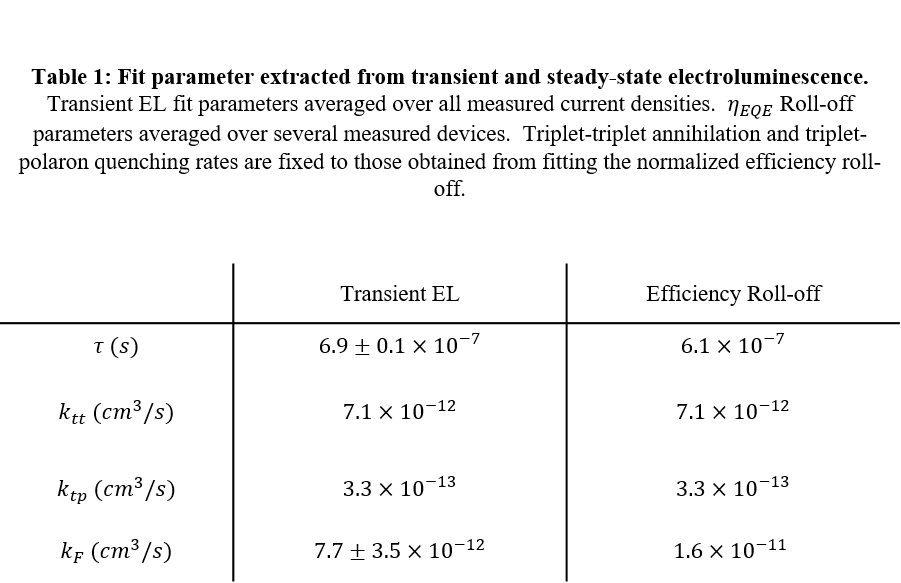
\includegraphics[scale=.25]{unified/valueTable}
\subsubsection{Term Efficiency During Transient}
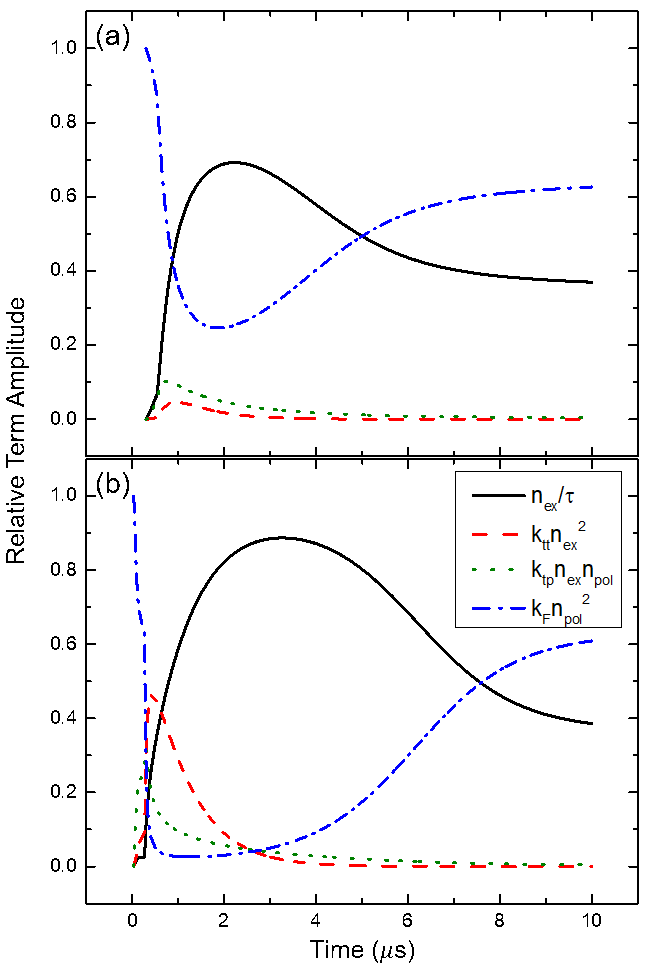
\includegraphics[scale=.25]{unified/termEfficiency}
\subsubsection{Extracting Exciton Formation Efficiency}
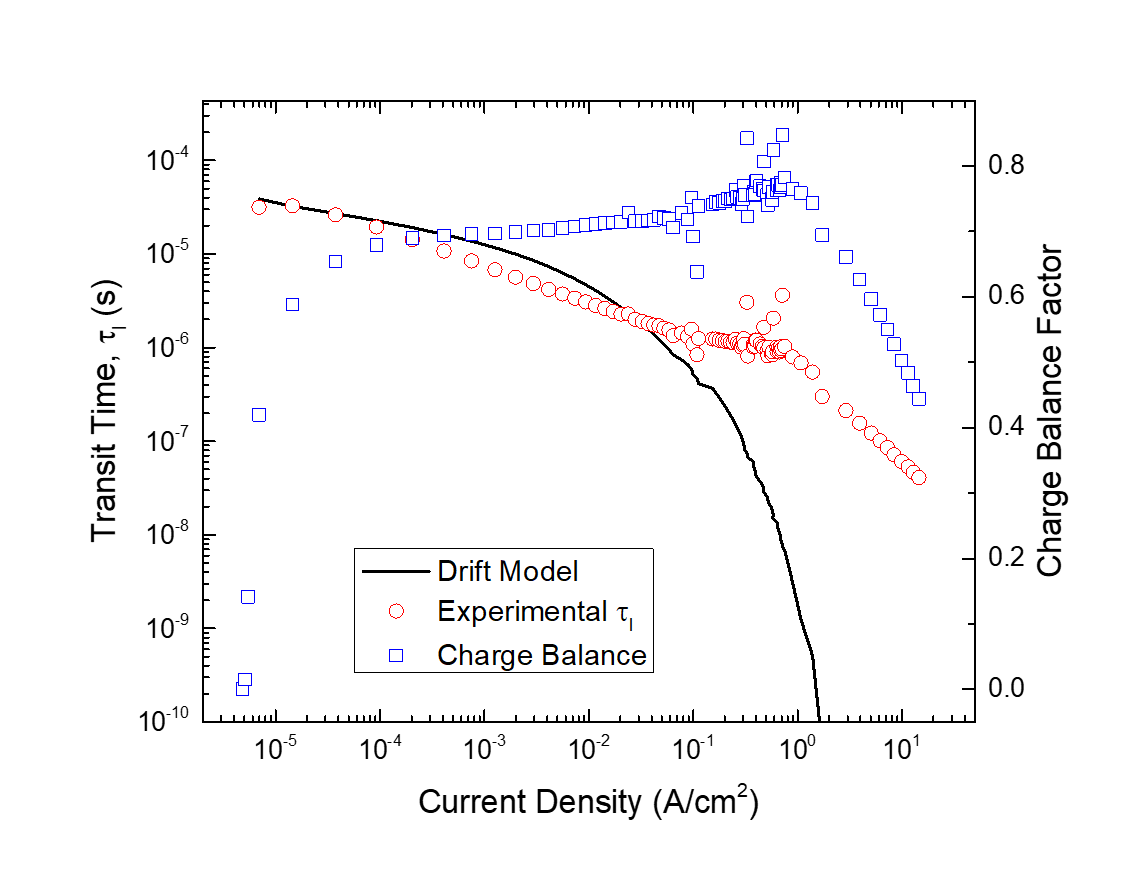
\includegraphics[scale=.25]{unified/chargeBalance}
\subsubsection{Drift Model}
\subsection{Understanding Assumptions of Polaron Model}
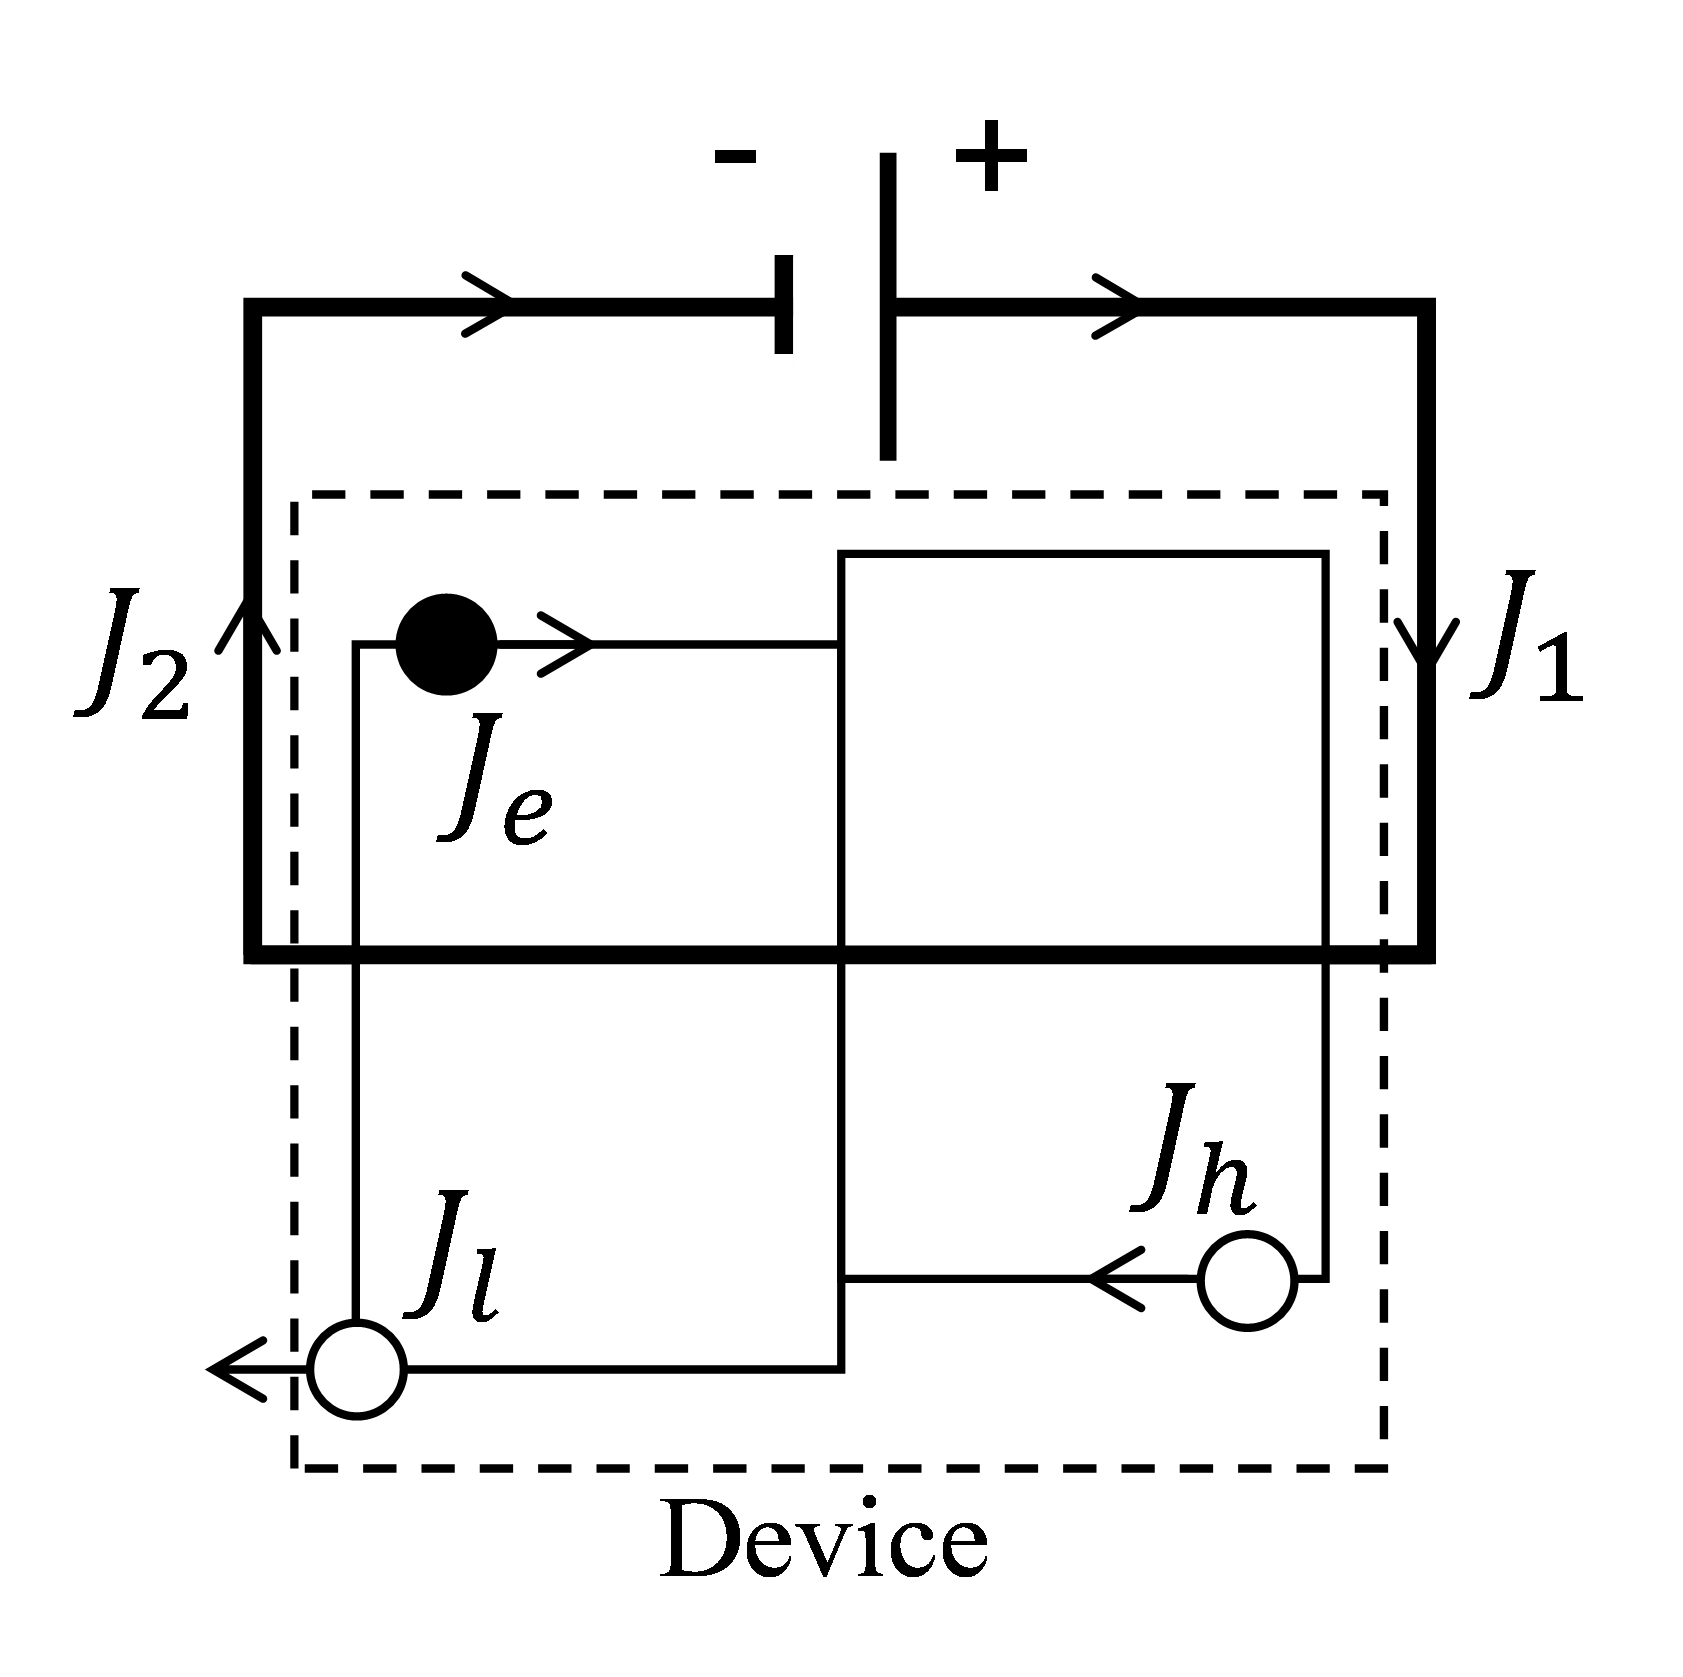
\includegraphics[scale=.1]{unified/currentDiagram}
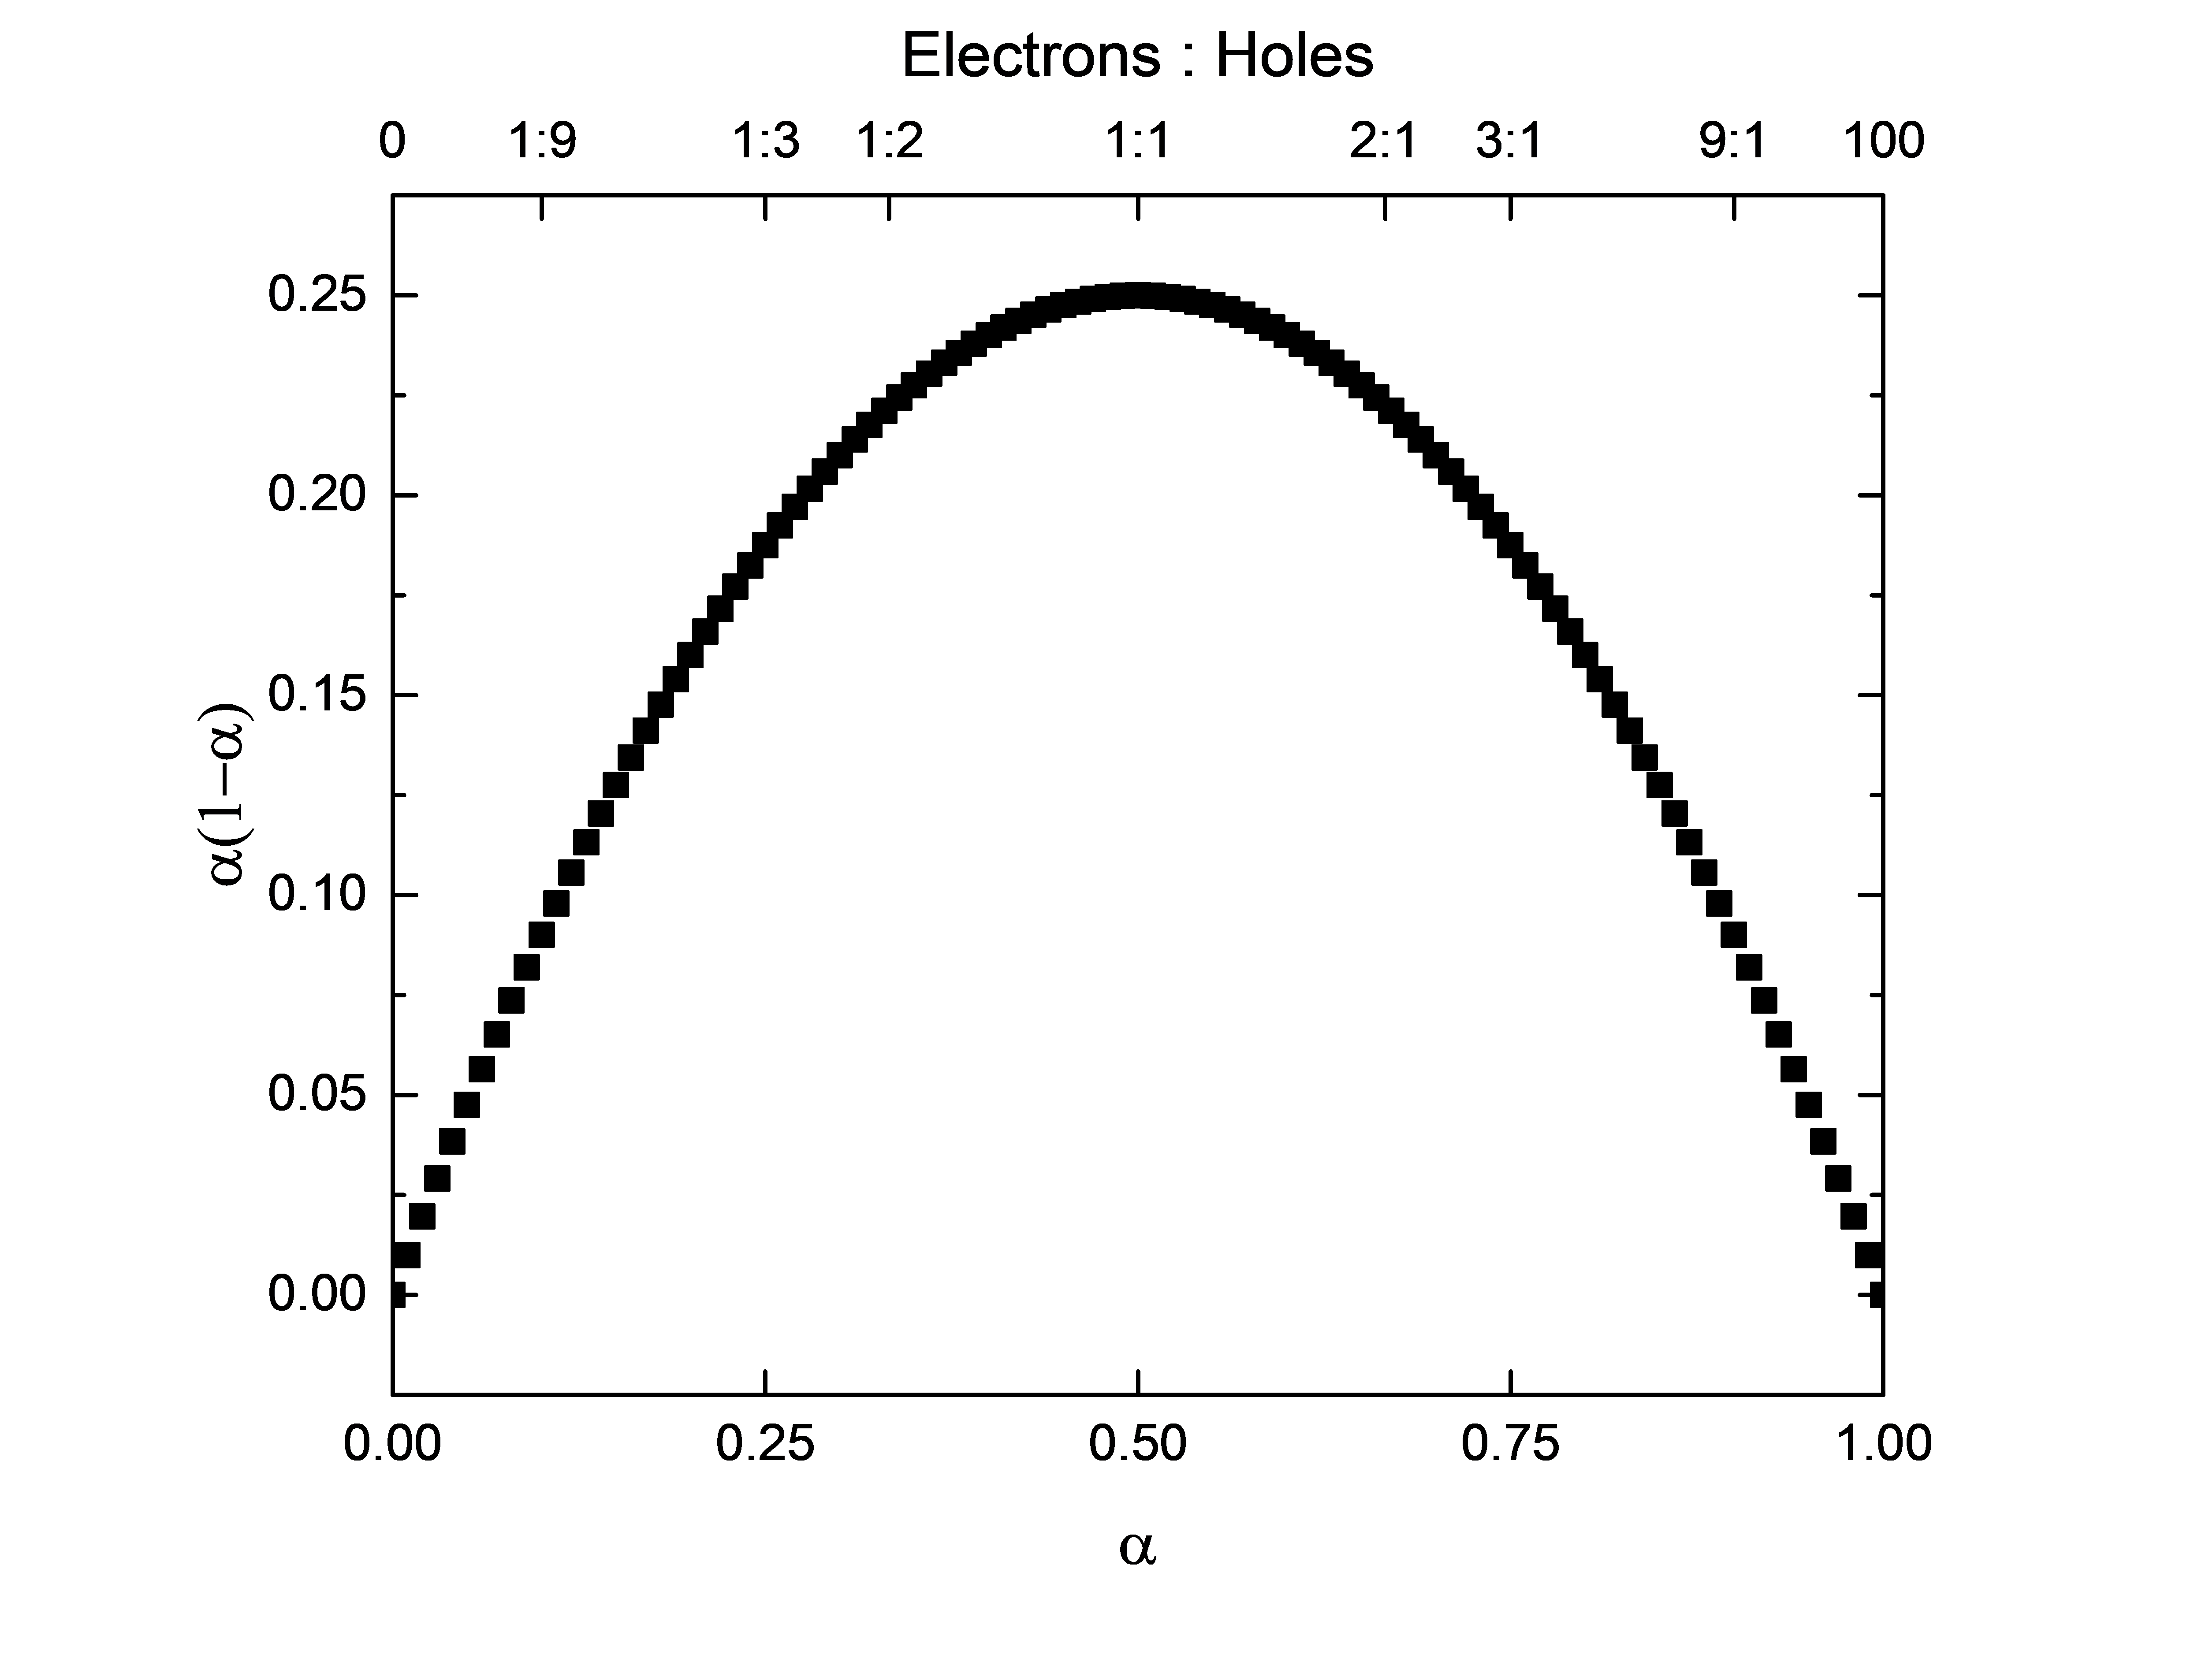
\includegraphics[scale=.1]{unified/EHratio}
\end{document}

